\chapter{The ATLAS track reconstruction chain}
\label{chap:atlas-reco-chain}

The High Luminosity era brings many challenges to event reconstruction in general and charged-particle tracking in particular, due to increased pile-up level and detector granularity. 
The current algorithm used in offline tracking scales super-linearly with pile-up and struggles to meet the future operational requirements. 
This motivates the development of an alternative algorithm that leverages modern hardware accelerators, such as the Graphic Processing Unit (GPU) or the Field-Programmable Gate Array (FPGA), to boost the reconstruction speed.
% The obvious questions arising when one proposes a new algorithm is: \textit{Does it perform the task as well as the existing algorithm?}, and \textit{if not, why?}. 
In this context, an understanding of the existing algorithm is necessary to adequately compare its performance to that of the proposed algorithm. 
% Answering such questions necessitates understanding of both the existing and the novel algorithms. 
This chapter describes the working principle of the Combinatorial Kalman Filter--the engine of charged-particle tracking, and the challenges facing it in the High-Lumnosity era.
The Kalman mechanism stems naturally from the least-square fit, which is also the basis of the discussion in chapter \ref{chap:tracking-performance}.

\section{Clusterization and space point formation}
\label{sect:cluster-spacepoint}

The first step of track reconstruction is the clusterization of the energy deposit on individual sensor cells recorded by the detector.
Figure \ref{fig:clustering} illustrates a particle passing through a planar pixel sensor and depositing a small amount of its energy. 
% the detector read-outs when a particle passes through a pixel module. 
Each sensor cell independently measures this energy and, when the energy exceeds a certain threshold, records a signal.
Throughout an event, a sensor may experience multiple passages of different particle trajectories, as shown on figure \ref{fig:sp-calcul}, so its collection of cell read-outs must then be sorted into groups of neighbouring cells likely to originate from the same particle. 
This process, called clusterization, transforms low-level information from individual sensor cells to a higher-level and more compact objects, called \textbf{clusters}. 

\begin{figure}[htb]
    \centering
        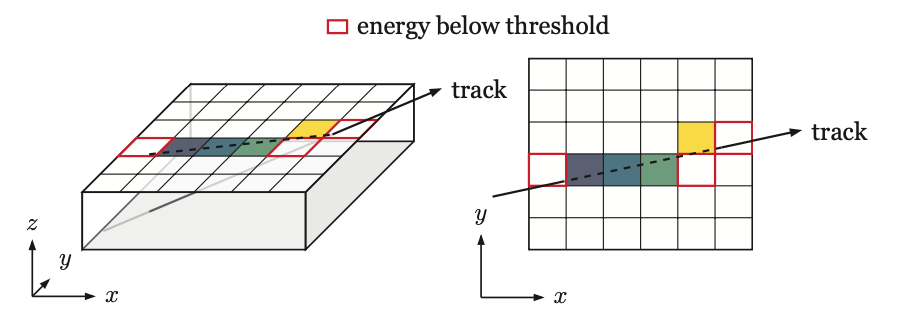
\includegraphics[width=0.8\textwidth]{figures/clustering.png}
    \caption{Formation of a pixel clusters from multiple cells. The particle deposits its energy in 7 cells, 5 of which receive charges exceeding the detection threshold and enter the clusterization \cite{paul-thesis}.}
    \label{fig:clustering}
\end{figure}

ATLAS traditionally uses a connected component analysis (CCA) \cite{CCA-pixel}, and more recently a neural network-based approach to clusterize cell read-outs\cite{clustering_nn}.
The intersection point $\mathbf{l}$ between the track and the sensor is estimated from the local coordinates $\mathbf{l}_i$ of each cells in the clusters
\beq
\label{eq:track-fit:1-1}
\mathbf{l} = \begin{cases}
    \frac{1}{N} \sum_i \mathbf{l}_i \\
    \frac{1}{\sum_i q_i} \sum_i q_i \mathbf{l}_i
\end{cases},
\eeq
where $q_i$ is the charge deposit on cell $i$. 
The first formula computes a simple vector mean of the cell location, and the second a charge-weighted mean. 
In the neural network approach, the cluster position and uncertainty are both predicted by the network and found to be more accurate than the (weighted) mean approach.

\begin{figure}[htb]
    \centering
        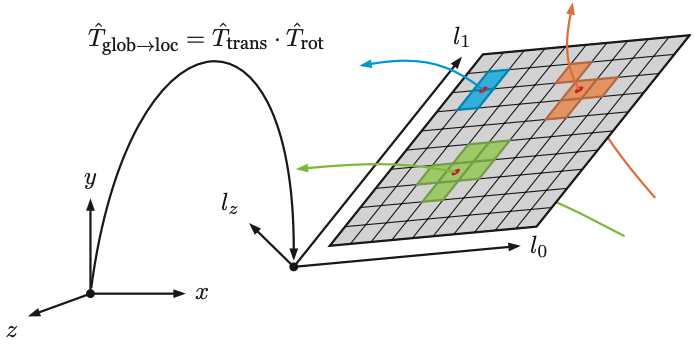
\includegraphics[width=0.8\textwidth]{figures/sp-calculation.png}
    \caption{The passage of a particle through a pixel sensor segmented in two dimensions. The energy deposit in each sensor cell is measured as a signal when it exceeds a measurement threshold. The true intersection point is estimated from the signal cells grouped together, called a cluster~\cite{paul-thesis}.}
    \label{fig:sp-calcul}
\end{figure}

A cluster can be regarded as a measurement made in the local coordinate of the measuring surface\footnote{For rest of this thesis, the terms ``measurement" and ``cluster" are interchangeable and refer to the same objects}.
From a cluster, the location of the hit in global coordinate, called the space point, can be derived.
Figure \ref{fig:sp-calcul} illustrates three particle tracks traversing a pixel sensor and inducing separate clusters. 
The true intersections are shown as red dots. 
An estimate of each of the true intersections between the trajectory and the sensor plane shown as red dots, is made in the clusterization step, and combined with the location and rotation of the sensor surface to obtain the space points.
In this sense, pixel space point formation is obtained from a change in reference frame of the cluster coordinates via a series of translational and rotational transformations. 

\begin{figure}[htb]
    \centering
    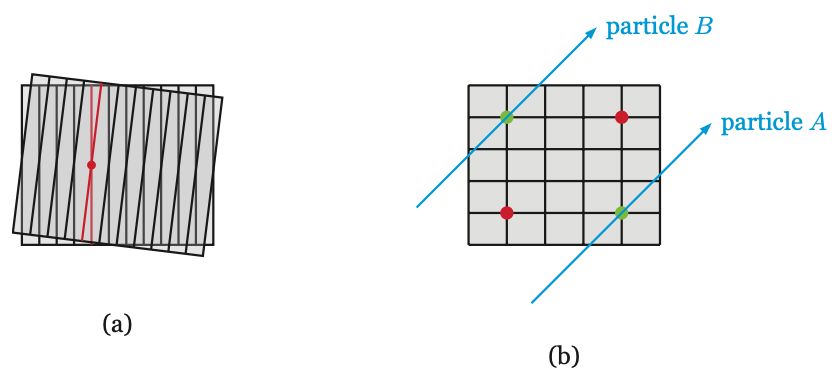
\includegraphics[width=0.8\linewidth]{figures/sp-calcul-strip.png}
    \caption{A pair of strip sensors are used to reconstruct a 3-dimensional estimate of the particle's true impact point (a). Ambiguity arises when more than one particle hit a strip module, leading to more combinations than particles (b) \cite{paul-thesis}. }
    \label{fig:sp-calcul-strip}
\end{figure}

While there is a one-to-one correspondence between a pixel cluster and a pixel space point, the space point formation in the strip detector is more complicated.
Strip modules are finely segmented in only one direction, rendering each measurement one-dimensional, in contrast to the two-dimensional measurements on a pixel module.
To obtain a three-dimensional position estimate, two strip clusters from the same layer are combined, as shown in fig. \ref{fig:sp-calcul-strip}. 
The local position of the hit along the thinly segmented dimension is estimated with high resolution.
Thanks to the stereo angle between the modules, an estimate of the second coordinate is made from the intersection of the strip cells, albeit with lower resolution. 
These measurements are then transformed to a global position estimate, as described above. 

% Ambiguity arises when multiple particles hit the same pair of strip modules, each generating two clusters, as shown on the left figure of \ref{fig:sp-calcul-strip}. 
% As the number of cluster combinations exceeds the number of particles, ghost space points are created by false association of clusters. 

In the current track reconstruction chain, space points are used to build track seeds, which are small groups of hits likely to originate from the same particle. 
A dedicated seeding stage creates large number of seeds each containing three space points and subsequently feeds them to a track building algorithm. 
The latter extends the seed by iteratively adding clusters that are compatible with the corresponding track state.
A small number of clusters in the final track candidate come from the seed space points, and the rest from individually incorporated clusters on the track path.

\begin{figure}[h!]
    \centering
    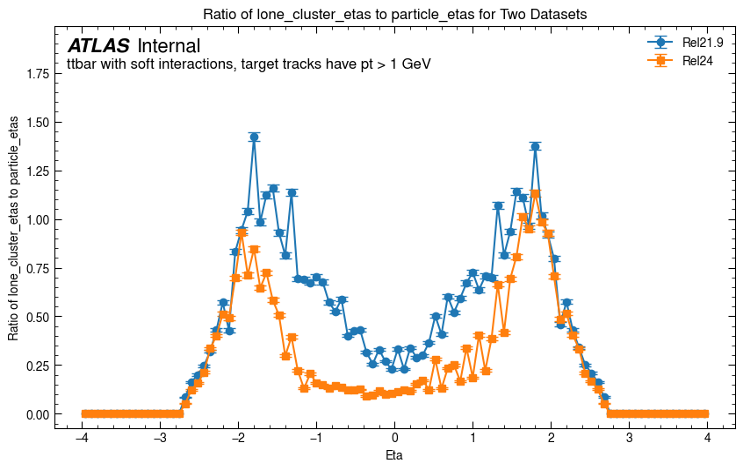
\includegraphics[width=0.7\textwidth]{figures/lone-clusters.png}    
    \caption{Average number of lone strip clusters per track as a function of the particle pseudorapdity $\eta$.}
    \label{fig:lone-cluster-distribution}
\end{figure}

Finally, we note an important consequence of the 2-cluster composition of the strip space point.
Despite meticulous optimization of the detector layout, a particle does not always leave two hits on a strip layer. 
Silicon sensors have inherent inefficiency, which means that a particle may traverse a detector module without inducing a signal.
This phenomenon occurs in both sub-detectors of the ITk, but is very unlikely.
A more important inefficiency comes from the the strip detector, in which a particle may approach a layer in a direction such that it intersects only one of two physical strip modules (see section \ref{sect:itk-overview} for a description of the strip detector). 
For any reason, when a strip layer records a \textit{lone} cluster, it is ignored by the space point formation algorithm, resulting in its absence from the space point collection.
On figure \ref{fig:lone-cluster-distribution}, we observe that particles leave lone clusters when their pseudorapdity falls under the coverage of the strip detector at $\abs{\eta}<2.8$, 
reaching up to one lone cluster per particle at $\abs{\eta}\simeq 1.8$.
This means that if we look at the space point record, every particle in this region effectively skips a strip layer.
This hit inefficiency is inconsequential in the current ATLAS reconstruction chain, because space points are only used for track seeding, and there is enough redundancy to cover all true particle seeds.
However, an algorithm that builds tracks from space points would not see lone clusters in the input, which may cause potential impacts on its performance.
This issue will become important for the new algorithm and be described in chapter \ref{chap:tracking-performance}.

\section{The least-square fit}
\label{sect:track-fit}

A track candidate is a set of measurements made by sensitive detector elements on the particle's trajectory. 
The latter is mathematically represented by a set of parameters describing its position and momentum as it traverses the detector. 
Although in idealized situations, the track may be parametrized by constants of motion, in a realistic detector, even these constants vary over time, due to random material effects. 
Therefore, a necessary ingredient to describe the trajectory is the solution to the equation of motion given the detector setup. 
From an initial value and the precise magnetic field on a dense grid of sampling points, the equation of motion is numerically integrated to obtain the a description of that particle state as it evolves along the trajectory. 

Let $\bfx\in \mathbb{R}^d$ represent the state of the particle and vary as a function of the arc length $s$ along the trajectory\footnote{Since $s=vt$, this is equivalent to parametrization in time.}, so that 
\beq
\label{eq:track-fit:1}
\bfx = \bfx(s)
\eeq
We will keep the discussion here general and note that any set of parameters from which the instantaneous position and momentum of the particle can be derived is usable. 
The choice of parametrization in ATLAS is discussed in section \ref{sect:chi2-fit}.
In general, track parameters can be regarded as the internal state of the particle, which is not directly measurable.
Instead the measurements are made at discrete points on the trajectory where a sensitive module is present.
Each measurement $\bfm_i$ can then be modelled as a deterministic function of the track state at that the measuring surface $\bfx_i$ superimposed by a random experimental noise $\epsilon_i$.
\beq
\label{eq:track-fit:2}
\bfm_i = h_i(\bfx_i) + \epsilon_i.
\eeq
The function $h_i:\mathbb{R}^d \rightarrow \mathbb{R}^n$, called the \textit{measurement model}, projects the $d$-dimensional state vector $\bfx_i$ on the $i$-th surface to an $n$-dimensional measurement vector. 
Its functional form depends on the type of measuring surface, hence the subscript.
For example, a measurement on a pixel module is intrinsically different from one on a strip module\footnote{A pixel cluster is a $2D$ measurement, while a strip cluster is $1D$.}, so their measurement models naturally differ. 

The experimental noise $\epsilon_i$ also depends on the type of measuring surface. 
However, it is generally assumed to be unbiased with finite variance, namely
\beq
\label{eq:track-fit:3}
E[\epsilon_i] = \mathbf{0}, \quad 0<\sigma(\epsilon_i^{(j)}) < +\infty ,\forall \, j \in [n],
\eeq
where the superscript denotes the $j$-th component of the $n$-dimensional error vector.
The covariance matrix of $\epsilon$ is an important ingredient of the least-square fit, denoted by
\beq
\label{eq:track-fit:4}
\mathbf{V}_i = E[\epsilon_i \epsilon_i ^T]
\eeq

As mentioned above, the state vector evolves along the trajectory, governed by the Equation of Motion (EOM), the solution to which is called the track model. 
The system evolution can be written as a recursive process
\beq
\label{eq:track-fit:5}
\bfx_i = \bfx(s_i) = f_{i-1} (\bfx_{i-1}).
\eeq
The extrapolation function $f_{i-1}: \mathbb{R}^d\rightarrow\mathbb{R}^d$ projects the track state from the previous measuring surface $\bfx_{i-1}$ to the current surface. 
Its functional form depends on the equation of motion, which in turns depends on detector characteristics, such as its magnetic field and layouts.
As the EOM is in general a second-order non-linear differential equation, a close-form solution, if it exists, is likely non-linear.
However, in practice, the EOM is often linearized and numerically integrated by, for example, Euler's method, allowing a linear, albeit recursive and potentially expensive solution
\beq
\label{eq:track-fit:6}
\bfx(s_{i-1} + \Delta s)\approx \bfx(s_{i-1}) +     \frac{\partial \bfx'}{ds'} \Big \vert _{s'=s_{i-1} }\Delta s + \mathcal{O}((\Delta s)^2),
\eeq
where the derivative is calculated from the dynamical equation of the system. 
More sophisticated numerical methods can be used, but in principle, it is possible to approximate the transport equation \eqref{eq:track-fit:5} as a linear recursive relation. 
The benefit of such linearization is that we can write the track state on any surface $\bfx_i $ as a simple linear function of some initial value on a reference surface $\bfx_0$,
\beq
\label{eq:track-fit:7}
\bfx_i = f_{i-1}(x_{i-1}) = f_{i-1}(f_{i-2}(\bfx_{i-2})) = f_{i-1} \circ f_{i-2} \circ \dotsc \circ f_0 (\bfx_0) = f_i (\bfx_0),
\eeq
and take $\bfx_0$ as \textit{the} estimated track parameters.

Track fitting is now reduced to finding an estimator $F$ from the set of measurements $M=\{\bfm_1,\dotsc,\bfm_N\}$ to the parameter space, such that (1) the estimate $\hat{\bfx}_0=F(M)$ is unbiased
\beq
\label{eq:track-fit:8}
E[\hat{\bfx}_0] = \bfx_0
\eeq
and (2) of minimum variance
\beq
\label{eq:track-fit:9}
E[(F(M) - \bfx_0)^2] = \min_{F'} E[(F'(M) - \bfx_0)^2]
\eeq
The Gauss-Markov theorem \cite{gauss-markov} states that among the class of linear and unbiased estimators, the Least Squares Estimator (LSE) has minimum variance, provided a linear track model, purely statistical\footnote{i.e. independent of $\bfx$}, unbiased and uncorrelated errors $\epsilon_i$. 
The LSE is obtained by minimizing the $\chi^2$-function, defined as
\beq
\label{eq:track-fit:10}
\chi^2 = \sum_{i=1}^N [\bfm_i - h_i(f_i(\bfx_0))]^T \mathbf{V}_i^{-1}[\bfm_i - h_i(f_i(\bfx_0))],
\eeq
where both $h_i$ and $f_i$ are now assumed to be linear.
The linearity of $h_i$ can be achieved by a careful choice of parametrization, such as the one used by ATLAS, discussed in section \ref{sect:chi2-fit}.
The estimator is simply the solution to
\beq
\label{eq:track-fit:11}
\nabla  \chi^2(\bfx_0) = 0
\eeq

\section{Iterative track fit}
\label{sect:kalman-filter}

Because the LSM considers all measurements at the same time, it is a global fitting method. 
It can be shown that in situations where the material effects described in section \ref{sect:material-effects} cannot be ignored, the minimization of the $\chi^2$-function translates to the inversion of a non-diagonal covariance matrix whose dimension grows with the number of measurements $N$. 
This computation can become a significant bottleneck in complex and granular detectors (see chapter 3 of reference \cite{Regler2000-ie} for more details).

The Kalman formalism \cite{Mankel_2004, BILLOIR1984352, FRUHWIRTH1987444} offers a faster alternative to global fit that, crucially, yields optimal estimates for Gaussian measurement uncertainties. 
The track state still evolves as a linear dynamical system.
Multiple scattering and energy loss due to material interactions are modelled as random process noise $\mathbf{w}$ added to the transport equation 
\beq
\label{eq:track-fit:12}
\bfx_i = \mathbf{F}_{i-1}\bfx_{i-1} + \mathbf{w}_{i-1},
\eeq
where the matrix $\mathbf{F}_{i-1}$ is the track model given in equation \eqref{eq:track-fit:5} now written in the explicitly linear form. 
The process noise $\mathbf{w}$ has a covariance denoted by
\beq
\label{eq:track-fit:13}
\mathbf{Q} = E[(\mathbf{w} - E[\mathbf{w}])(\mathbf{w} - E[\mathbf{w}])^T]
\eeq
Instead of minimizing a $\chi^2$-function over all measurements, the Kalman procedure iteratively incorporates measurements into an existing estimate of the track parameters. 
Each iteration inverts a single $n\times n$ matrix, so in total, $N$ inversions of $n\times n$-matrices are needed, where $n$ is the number of measurement coordinates\footnote{In typical ATLAS parametrization, $n=2$} and $N$ the number of measurements, as opposed to inverting an $(nN)\times (nN)$ matrix in the LSM.
The information from the measurement is used to constrain the estimate and reduce the error. 
The procedure is carried out in the following 3-step recipe. \\
\textbf{Step 1: Prediction}. Suppose the measurement $\bfm_i\in M$ is being incorporated. 
Let $\bfx_{i-1}$ and $x_{i}^{i-1}$ denote the track state before the inclusion of $\bfm_i$, and its projection to the measuring surface of $\bfm_i$ by the transport equation.
In addition, denote the covariance of the estimate as $\mathbf{C}$,
\beq
\label{eq:track-fit:13-1}
\mathbf{C} = E[(\bfx - E[\bfx])(\bfx - E[\bfx])^T],
\eeq
so that the covariance before inclusion is $\mathbf{C}_{i-1}$.
\textit{Neither} of $\bfx_{i-1}$ nor $\bfx_i^{i-1}$ contains information from $\bfm_i$, nor any material effect during the propagation, 
\beq
\label{eq:track-fit:14}
\bfx_i^{i-1} = \mathbf{F}_{i-1}\bfx_{i-1}.
\eeq
The stochastic noise due multiple Coulomb scattering and energy loss corrections is instead superimposed on the projected covariance,
\beq
\label{eq:track-fit:16}
\mathbf{C}_i^{i-1} = \mathbf{F}_{i-1}\mathbf{C}_{i-1}\mathbf{F}_{i-1}^T + \mathbf{Q}_{i-1}.
\eeq
\textbf{Step 2: Filtering}. The predicted track state in \eqref{eq:track-fit:14} is combined with the present measurement $\bfm_i$ to yield the updated estimate $\bfx_i$ 
\beq
\label{eq:track-fit:17}
\bfx_i = \bfx_i^{i-1} + \mathbf{K}_i(\bfm_i - \mathbf{H}_i\bfx_i^{i-1}).
\eeq
$\mathbf{K}_i$ is called the Kalman gain matrix 
\beq
\label{eq:track-fit:18}
\mathbf{K}_i = \mathbf{C}_i^{i-1}\mathbf{H}_i^T(\mathbf{V}_i + \mathbf{H}_i\mathbf{C}_i^{i-1}\mathbf{H}_i^T)^{-1}.
\eeq
Intuitively, $(\bfm_i - \mathbf{H}_i\bfx_i^{i-1})$ represents the difference between the actual measurement and the expected measurement given the predicted track state.
If the measurement exactly equals its predicted value, it supports the predicted track state, so the update track state equals its predicted value.
No new information is added to the filtered estimate in such a case.
Therefore, we can think of the Kalman matrix as the information gained from any disagreement between the predicted and the actual measurement, hence its denomination. 

The covariance of the estimate is updated from its prediction as
\beq
\label{eq:track-fit:19}
\mathbf{C}_i = (\mathbf{I} - \mathbf{K}_i\mathbf{H}_i)\mathbf{C}_i^{i-1}.
\eeq
The uncertainty from stochastic noise and the measurement uncertainty are respectively encoded in $\mathbf{C}_i^{i-1}$ and $\mathbf{K}_i$. 
Both sources of uncertainty thus contribute to the filtered covariance, as expected.
Both the state vector and its covariance are updated by incorporating a new measurement and the material effects from propagating the particle from its last known position.

Repeated applications of prediction and filtering incorporate all measurements to refine the track state from its initial value $\bfx_0$ \\
\textbf{3. Smoothing}. The prediction and filtering sequence refines the track state in the forward direction.
This means that an estimate at the end of the trajectory is better than one at the beginning. 
It is, however, desirable that all estimates receive information from all measurements, rather than those preceding them. 
The smoothing step achieves this goal by working backward from the outermost measurement and updating a state vector at step $i$ using the state vector at step $i+1$
\beq
\label{eq:track-fit:20}
\bfx_i^N = \bfx_i + \mathbf{A}_i(\bfx_{i+1}^N - \bfx_{i+1}^i),
\eeq
in which the superscript $N$ signifies an estimate incorporating all $N$ measurements. 
$\mathbf{A}_i$ is called the smoothing gain matrix, defined as
\beq
\label{eq:track-fit:21}
\mathbf{A}_i = \mathbf{C}_i \mathbf{F}_i^T(\mathbf{C}_{i+1}^i)^{-1}.
\eeq
Only after filtering through all measurements on track can the smoothing be effected. 
In ATLAS terminology, the former is therefore referred to as the forward filter, while the latter backward smoothing.
The initial track state $\bfx_0$, or the state on any other surface, real or imaginary, can be refined or extrapolated using the entire measurement set. 

% [Discuss the connection to the minimum variance principle here, and mention the global chi2 under the hood]

\section{Combinatorial Kalman Filter}
\label{sect:CKF}
Thanks to its iterative mechanism, the Kalman formalism can be extended from track fitting to track finding, called the Combinatorial Kalman Filter (CKF). 
From a track seed containing $k$ measurements, it estimates the initial value $\bfx_k$ and projects it to the next surface using equation \eqref{eq:track-fit:12}.
In the filtering stage, instead of incorporating a given measurement, as in the case of track fitting, it considers all measurements on the target surface falling into a search window defined by the projected measurement covariance.
By filtering each candidate measurement $l$, it computes a filtered track state and measurement residual
\beq
\label{eq:track-fit:22}
\mathbf{r}_{k+1, l} = \bfm_{k+1, l} - \mathbf{H}_{k+1}\bfx_{k+1, l}.
\eeq
The increment in $\chi^2$ is computed from the residual
\beq
\label{eq:track-fit:23}
\chi^2_{+, l} = \mathbf{r}_{k+1, l}^T[(\mathbf{I} - \mathbf{H}_{k+1}\mathbf{K}_{k+1}) \mathbf{V}_{k+1, l}]^{-1} \mathbf{r}_{k+1, l}.
\eeq
All candidate measurements $l$ whose contribution to the global $\chi^2$ falls before a certain threshold are admitted, creating the same number of branches from the track seeds.
The procedure is repeated till no more measurements can be incorporated. 
The output from a given track seed is usually a large set of track candidates each originating from a combination of branching connections, hence the \textit{combinatorial} denomination.

The track candidate is characterized by a global $\chi^2$ equal to the sum of the contributions from individual measurements in equation \eqref{eq:track-fit:23}.
Several candidates might be ruled out based on the mean $\chi^2_{track} / \abs{M_{track}}$, as well as other quality cuts. 
To guarantee tracking efficiency, a large number of track seeds are produced and considered by the CKF.
The number of considered track seeds combined with the number of combinations per seed results in significant track redundancy and overlapping measurements. 
An ambiguity resolution step globally sorts through the track candidates and assigns each measurement to mostly a unique track, effectively reducing them to a set of tracks of highest quality and compatibility to real particles. 

\section{Computational cost of track reconstruction}
\label{sect:computational-cost-ckf}

Inner tracking is one of the most expensive tasks of event reconstruction. 
For instance, table \ref{tab:reco-time-breakdown} illustrates the CPU consumption in \hssec~of each reconstruction stage under Run 2 conditions but scaled to $\expval{\mu}=90$ \cite{CERN-LHCC-2020-015}.
Track reconstruction dominates the computing budget, consuming $67\%$ of the total reconstruction time.
This contribution will only get worse at pile-up 200, due to the strong scaling behaviour of the Combinatorial Kalman Filter and the Ambiguity Resolution step which necessarily follows.

\begin{table}[h!]
    \centering
    \begin{tabular}{|c|c||c|c|c|c||c|}
    \hline
       Detector  & $\expval{\mu}$ & Tracking & Calo and M.S & Combined Reco. & Monitoring &  Total \\
       \hline
        Run 2 & 90 & 1137 & 149 & 301 & 106 & 1693 \\ \hline
    \end{tabular}
    \caption{The CPU required in \hssec~to reconstruct a Run 2 data event using the corresponding software release at average pile-up 90 using. The total reconstruction time is broken down into inner tracking, Calorimeter and Muon Spectrometer reconstruction, and Monitoring. Numerical figures taken from reference \cite{CERN-LHCC-2020-015}.}
    \label{tab:reco-time-breakdown}
\end{table}

Within Inner Tracking, the tracking finding step described in this chapter consumes the largest CPU resource. 
Listed in table \ref{tab:tracking-time-breakdown} are the cost of each step in the tracking stage, assuming the pile-up levels of 140 and 200. 
In the default tracking chain, the tracking finding and ambiguity resolution steps dominate the total CPU consumption. 
Although listed as separate items, the former's performance is severely degraded without the latter, so they should be considered together as one item, which occupies $83\%$ of the overall computing consumption for inner tracking at pile-up 200.

\begin{table}[h!]
    \centering
    \begin{tabular}{|c|c||c|c|c|c|c||c|}
    \hline
       $\expval{\mu}$  & Algorithm & Decoding & Clustering & S.P. Formation & CKF & Am. Reso. &  Total \\
       \hline \hline
        140 & Default & 1.2 & 17.1 & 6.0 & 41.1 & 58.2 & 124 \\ \hline
        140 & Fast & 1.2 & 4.5 & 0.9 & 12.4 &  & 19.0 \\ \hline \hline

        200 & Default & 1.6 & 26.3 & 8.6 & 85.8 & 92.0 & 214 \\ \hline
        200 & Fast & 1.6 & 6.3 & 1.2 & 22.6 & & 31.7 \\ \hline
    \end{tabular}
    \caption{The CPU required in \hssec~to reconstruct a $t\bar{t}$ MC event with $\expval{\mu}=140$ and 200 in the ITk. The total track reconstruction time, evaluated for both the default and an optimized CKF-based chains, is broken down into individual steps, most significant of which are clustering, space point formation, CKF-based track finding and ambiguity resolution. An Intel Xeon E5-2620v2 processor with 2.1 GHz and six physical cores per CPU was used. The CPU time is multiplied by an HS06 factor of 17.8 for single-thread running. Numerical figures taken from reference \cite{ATL-PHYS-PUB-2019-041}.}
    \label{tab:tracking-time-breakdown}
\end{table}

ATLAS has carried out major optimizations of the default CKF chain to improve its CPU performance, shown in table \ref{tab:tracking-time-breakdown} as Fast tracking. 
Track seeds used to initialize the CKF are created exclusively from pixel space points, enabled by the increased number of expected pixel hits thanks to an additional layer and the full $\eta$-coverage of the ITk compared to the ID. 
A tighter track selection and precise cluster calibrations are used to remove duplicate and fake tracks after the track finding step, in lieu of the costly ambiguity resolution step. 
These changes, along with other incremental improvements, allows running the track reconstruction pass approximately 8 times faster than the default chain, as illustrated in table \ref{tab:tracking-time-breakdown}, but with a loss in physics performance, as shown in figure \ref{fig:fast-default-phys} \cite{ATL-PHYS-PUB-2019-041}.
Despite the impressive acceleration, the fast track chain still is far from ready for production due to both latency and tracking performance.

\begin{figure}[t]
    \centering
    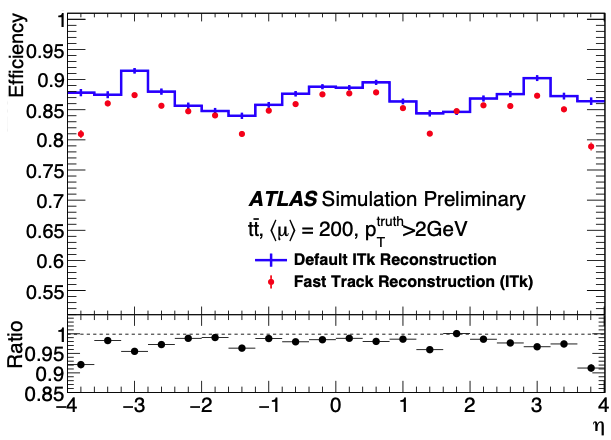
\includegraphics[width=0.49\textwidth]{figures/eff-fast-def.png}
    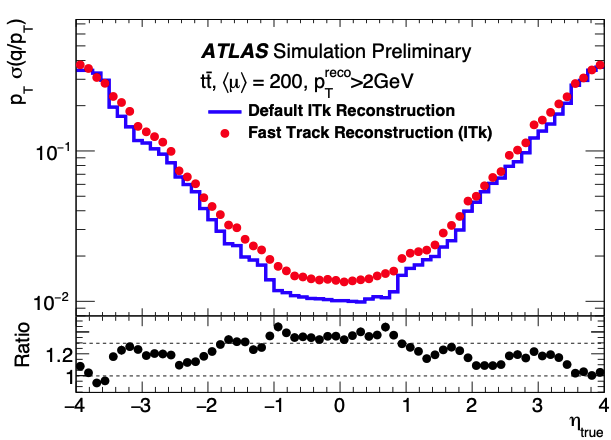
\includegraphics[width=0.49\textwidth]{figures/res-fast-def.png}
    \caption{Tracking efficiency (left) and track parameter resolution (right) as functions of the truth particle's pseudorapidity, evaluated at $\expval{\mu}=200$. The bottom plots show the ratio of the corresponding metric observed in the fast chain to that in the default chain~\cite{ATL-PHYS-PUB-2019-041}.}
    \label{fig:fast-default-phys}
\end{figure}

Along with optimizing the traditional event reconstruction algorithm, ATLAS is actively pursuing significant modernization of its analysis software, both online and offline. 
As outlined in reference \cite{CERN-LHCC-2022-005}, the primary challenge of the HL-LHC era will be the effective use of General Purpose Graphics Processing Units (GP-GPUs), which are becoming ubiquitous in large High-Performance Computing (HPC) facilities and data centers.  
They can accelerate suitable applications by orders of magnitude, many of which have already been deployed in ATLAS. 
Examples include Fast Simulation \cite{atlfast}, Particle Flow \cite{particle-flow}, and $b$-tagging graph neural networks \cite{GN1}.
Exploiting this computing resource requires recasting current software on the hardware accelerators, for instance the \hyperlink{https://github.com/acts-project/traccc}{\textsc{TrackCC}} project~\cite{andreas_salzburger_2025_15260074}, or designing new algorithms inherently compatible with them.
In addition, because of the increased track multiplicity in HL-LHC, online applications such as trigger and data acquisition will likely be migrated to accelerators, and thus, new hardware-accelerated algorithms are further incentivized for offline software to maintain synergies between the two computing domains.
In this context, the next big component in event reconstruction to be modernized is inner tracking, attracting substantial interest and investment in person power within ATLAS.
The work done in this thesis plays a significant role in this effort, resulting in a competitive candidate for an end-to-end, machine learning-based and fully GPU-compatible algorithm for track reconstruction. 
The remaining chapters of this thesis describe its development and latest results.

% For example, in a homogeneous magnetic field and no material interaction, the track model is a helical orbit with radius $R_{H}=\frac{p_T}{kqB}$ specified by an initial position $\mathbf{r}_0$ and momentum $\mathbf{p}_0$. 
% The magnetic field in ATLAS is far too complex for such an analytical solution to exist. In addition, interactions with detector material deviate the trajectory further from a perfect helix, and, as a result, the track model must be obtained from numerical integrations. 


% \section{Ambiguity Resolution}

% \section{The cost of tracking}

% \section{Summary}